\chapter{界面、表面活性剂与胶体}\label{ch:b3:colloids}

蛋黄酱是油以直径约几微米的液滴形式分散于少量
水和醋中，由蛋黄中的卵磷脂和蛋白质隔开。起初搅拌过快，
或油倒入过快，体系便会分为
油层与水层：液滴相互合并，维持液滴分开的
能量随之消失。牛奶、雾、墨水、油漆、血液以及河中的浑水，
都属于同一类物质：颗粒或液滴远大于分子，
却远小于肉眼所能见的任何物体，数量之多，使其中大部分分子
都靠近界面。本章讨论界面的能量、
降低界面能的分子、界面所促成的\omterm{def:b3:colloids:colloid}{胶体}，以及
使\omterm{def:b3:colloids:colloid}{胶体}保持分散或发生\omterm{def:b3:colloids:stability}{聚沉}的因素。

\begin{recall}
本科一年级分册把具有亲水头部和疏水尾部的分子称为两亲分子，
并讨论了色散力以及溶剂的
相对介电常数；第 1 册的十一年级部分在肥皂中认识了\omterm{def:b3:colloids:micelle}{胶束}。
本科二年级分册定义了化学势、离子强度和
活度。\Cref{ch:b3:surfaces-catalysis}讨论了固体表面的\omterm{def:b3:surfaces-catalysis:adsorption}{吸附}，
\cref{ch:b3:electrode-kinetics}讨论了\omterm{def:b3:electrode-kinetics:double-layer}{双电层}及其\omterm{def:b3:electrode-kinetics:double-layer}{德拜
长度}。物理学中的布朗运动，以及弯曲
表面内部的压强。
\end{recall}

\begin{omfigure}
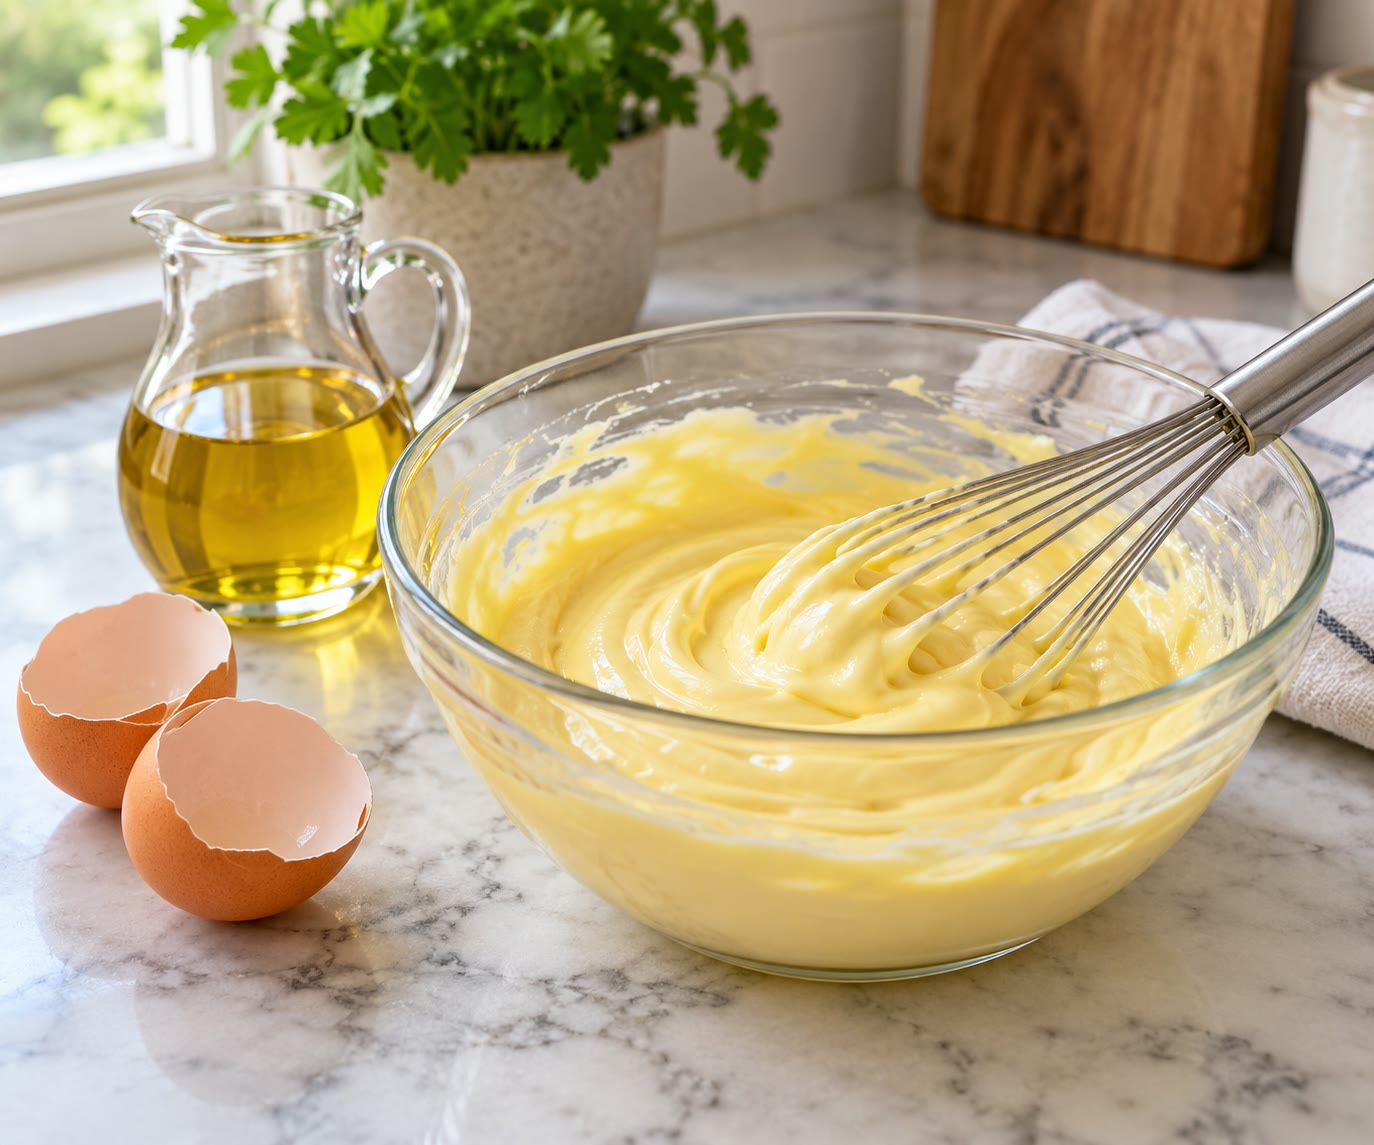
\includegraphics[width=0.6\linewidth]{images/book4/ai/b3-17-mayonnaise.jpg}

{\small 搅拌中的蛋黄酱：油滴分散于水中形成的\omterm{def:b3:colloids:colloid}{乳液}，
由蛋黄中的\omterm{def:b3:colloids:surfactant}{表面活性剂}稳定。}
\end{omfigure}

\section{界面与表面张力}

液体内部的分子在各个方向上受到的吸引相等；处于
表面的分子则失去部分近邻。形成表面需要消耗能量。

\begin{definition}[表面张力]\label{def:b3:colloids:surface-tension}
液体的\emph{表面张力}\index{表面张力} $\gamma$ 是指
在恒定温度、压强和组成下，产生单位面积表面所需的吉布斯自由能，
$\gamma = (\partial G/\partial A)_{T,p,n}$，单位为 \unit{J.m^{-2}} $=$ \unit{N.m^{-1}}。对于
两相之间的界面，则为界面张力。
\end{definition}

水靠氢键相互结合，\omterm{def:b3:colloids:surface-tension}{表面张力}较大：\qty{72.0}{mN/m}
在 \qty{25}{\celsius} 时；烷烃约为 20，汞约为 480。

\begin{proposition}[拉普拉斯压强]\label{prop:b3:colloids:laplace}
半径为 $r$ 的球形液滴或气泡内部的压强，
比外部压强高出的量为
\[
  \Delta p = \frac{2\gamma}{r} .
\]
\end{proposition}

\begin{proof}
平衡时将半径增加 $\dd r$，压强差所做的功
$\Delta p\,4\pi r^2\dd r$，等于表面吉布斯自由能的增量 $\gamma\,8\pi r\,\dd r$。
\end{proof}

\begin{definition}[接触角、润湿]\label{def:b3:colloids:wetting}
固体上液滴的\emph{接触角}\index{接触角} $\theta$ 是指一个角，
沿液体一侧量取，位于固体表面与液体表面之间，
其顶点位于固、液、气三相交线处。液体\emph{润湿}\index{润湿}
固体的条件是 $\theta < 90^\circ$，若 $\theta = 0$ 则完全铺展。
\end{definition}

\begin{theorem}[杨氏方程]\label{thm:b3:colloids:young}
平衡时，三个界面张力与\omterm{def:b3:colloids:wetting}{接触角}满足
\[
  \gamma_{\mathrm{SV}} = \gamma_{\mathrm{SL}} + \gamma_{\mathrm{LV}}\cos\theta .
\]
此即\emph{杨氏方程}\index{杨氏方程}。
\end{theorem}

\begin{proof}
将接触线向外移动 $\dd x$（沿单位长度接触线）：固–气
面积为 $\dd x$ 的固–气界面被固–液界面取代，而
液–气界面增加 $\dd x\cos\theta$。吉布斯自由能的变化为
$(\gamma_{\mathrm{SL}} - \gamma_{\mathrm{SV}} + \gamma_{\mathrm{LV}}\cos\theta)\dd x$，平衡时其值为零。
\end{proof}

\begin{omfigure}
\begin{tikzpicture}[font=\small, >=Stealth]
  \fill[black!12] (-3.6,-0.5) rectangle (3.6,0);
  \draw[thick] (-3.6,0) -- (3.6,0);
  \node[anchor=north] at (2.6,-0.05) {固体};
  \fill[omWater!60] (-2.0,0) arc[start angle=160, end angle=20, radius=2.13] -- cycle;
  \draw[thick, omDef] (-2.0,0) arc[start angle=160, end angle=20, radius=2.13];
  % circle centre 0.73 below the solid: a cap smaller than a hemisphere, contact angle 90 - 20 = 70 deg;
  % at the right contact point the liquid surface leaves at 110 deg (up and to the left)
  \draw[->, thick, omThm] (2.0,0) -- ++(110:1.3) node[anchor=south] {$\gamma_{\mathrm{LV}}$};
  \draw[->, thick] (2.0,0) -- (3.3,0) node[anchor=south] {$\gamma_{\mathrm{SV}}$};
  \draw[->, thick] (2.0,0) -- (0.7,0) node[anchor=north, yshift=-1pt] {$\gamma_{\mathrm{SL}}$};
  \draw (1.45,0) arc[start angle=180, end angle=110, radius=0.55];
  \node at (1.33,0.42) {$\theta$};
  \node at (0,0.6) {液体};
  \node at (-2.8,1.4) {蒸气};
\end{tikzpicture}

{\small 固着液滴及其接触线上受到的三种张力：
三者沿固体方向的分量平衡，即得\omterm{thm:b3:colloids:young}{杨氏方程}；此处 $\theta
\approx 70^\circ$，为部分\omterm{def:b3:colloids:wetting}{润湿}的液体。}
\end{omfigure}

\begin{theorem}[开尔文方程]\label{thm:b3:colloids:kelvin}
半径为 $r$ 的球形液滴的蒸气压，超过平面
液体的蒸气压 $p^*$：
\[
  \ln\frac{p}{p^*} = \frac{2\gamma V_{\mathrm m}}{rRT},
\]
其中 $V_{\mathrm m}$ 为液体的摩尔体积。此即\emph{开尔文
方程}\index{开尔文方程}。
\end{theorem}

\begin{proof}
液滴内的液体承受额外压强 $2\gamma/r$，这使其
化学势升高 $V_{\mathrm m}\,2\gamma/r$（此处 $(\partial\mu/\partial p)_T = V_{\mathrm m}$，液体不可压缩）。
与之平衡的蒸气，其化学势也必须升高
同样的量：$RT\ln(p/p^*) = 2\gamma V_{\mathrm m}/r$。
\end{proof}

对半径为 \qty{10}{nm}、温度为 \qty{25}{\celsius} 的水滴，$2\gamma V_{\mathrm m}/rRT = 0.105$：其蒸气压
比平面水高出 11\,\%。小液滴蒸发，
大液滴则长大；云的形成需要凝结核才能开始，小晶体的
溶解度同样遵循这一规律。

\begin{definition}[奥斯特瓦尔德熟化]\label{def:b3:colloids:ripening}
\emph{奥斯特瓦尔德熟化}\index{奥斯特瓦尔德熟化}是指分散体系中较大的
颗粒或液滴以牺牲较小颗粒为代价而长大的过程，其驱动力是
小颗粒具有较高的溶解度或蒸气压。
\end{definition}

\section{表面活性剂与胶束}

\begin{definition}[表面活性剂]\label{def:b3:colloids:surfactant}
\emph{表面活性剂}\index{表面活性剂}是一类两亲分子，它在界面上
\omterm{def:b3:surfaces-catalysis:adsorption}{吸附}并降低界面张力。若其头部为阴离子，则称为
\emph{阴离子表面活性剂}\index{阴离子表面活性剂}（如十二烷基硫酸钠、肥皂）；若
头部为阳离子，则称为\emph{阳离子表面活性剂}\index{阳离子表面活性剂}（如季铵盐）；若
头部为中性极性基团，则称为\emph{非离子表面活性剂}\index{非离子表面活性剂}，
例如由环氧乙烷单元组成的
链。
\end{definition}

\begin{definition}[表面过剩浓度]\label{def:b3:colloids:surface-excess}
溶质的\emph{表面过剩浓度}\index{表面过剩浓度} $\Gamma$ 是
单位面积界面上溶质的量，超出同一体积内
若本体浓度一直延伸到界面处时所能容纳的
量的部分。
\end{definition}

\begin{theorem}[吉布斯吸附等温式]\label{thm:b3:colloids:gibbs-adsorption}
对于浓度为 $c$ 的非离子型溶质稀溶液，
\[
  \Gamma = -\frac{1}{RT}\frac{\dd\gamma}{\dd\ln c};
\]
对于不加盐的 1:1 型离子\omterm{def:b3:colloids:surfactant}{表面活性剂}，$RT$ 应替换为 $2RT$。此即
\emph{吉布斯吸附等温式}\index{吉布斯吸附等温式}。
\end{theorem}

\begin{proof}
对于界面，在恒定 $T$ 和
$p$ 下，吉布斯–杜亥姆关系的类比形式为 $\dd\gamma = -\sum_i\Gamma_i\,\dd\mu_i$（表面吉布斯能 $\gamma A$ 起 $G$ 的作用，
此处承认）。选取分界面使溶剂的过剩量为零，
则 $\dd\gamma = -\Gamma\,\dd\mu$，而在稀溶液中 $\dd\mu = RT\,\dd\ln c$。对于离子型\omterm{def:b3:colloids:surfactant}{表面活性剂}，
阳离子和阴离子都以相等的过剩量\omterm{def:b3:surfaces-catalysis:adsorption}{吸附}，$\dd\mu$ 变为
$2RT\,\dd\ln c$.
\end{proof}

若\omterm{def:b3:colloids:surface-tension}{表面张力}随 $\ln c$ 线性下降，则
表面过剩为常数：界面已饱和，且 $1/(\Gamma N_A)$ 即为
每个\omterm{def:b3:surfaces-catalysis:adsorption}{吸附}分子所占的面积。

\begin{method}[由 $\gamma$--$\ln c$ 斜率求每个分子的面积]\label{met:b3:colloids:surface-excess}
\begin{enumerate}
  \item 在\omterm{def:b3:colloids:micelle}{临界胶束浓度}以下测量 $\gamma$ 随 $c$ 的变化，以 $\gamma$ 对 $\ln c$ 作图。
  \item 取\omterm{def:b3:colloids:micelle}{临界胶束浓度}以下线性部分的斜率；$\Gamma = -\text{斜率}/(nRT)$，$n
        = 1$ 对应\omterm{def:b3:colloids:surfactant}{非离子表面活性剂}，对不加盐的 1:1 型离子\omterm{def:b3:colloids:surfactant}{表面活性剂}为 2。
  \item 每个分子的面积 $= 1/(\Gamma N_A)$；典型值为 0.3 至 \qty{0.6}{nm^2}。
\end{enumerate}
\end{method}

\begin{definition}[胶束、临界胶束浓度、聚集数]\label{def:b3:colloids:micelle}
\emph{胶束}\index{胶束}是溶液中\omterm{def:b3:colloids:surfactant}{表面活性剂}分子形成的聚集体，
其疏水尾部构成类液体的内核，并被亲水头部与水隔开。
\emph{临界胶束浓度}\index{临界胶束浓度}（CMC）是胶束开始形成时
所对应的浓度；胶束所含分子的平均数目
称为\emph{聚集数}\index{聚集数}。
\end{definition}

\begin{proposition}[临界胶束浓度处的转折]\label{prop:b3:colloids:cmc-break}
高于\omterm{def:b3:colloids:micelle}{临界胶束浓度}时，游离\omterm{def:b3:colloids:surfactant}{表面活性剂}的浓度，以及随之而来的\omterm{def:b3:colloids:surface-tension}{表面
张力}和渗透压几乎保持不变；依赖于游离分子的性质
则在\omterm{def:b3:colloids:micelle}{临界胶束浓度}处改变斜率。
\end{proposition}

\begin{proof}[部分证明]
将\omterm{def:b3:colloids:micelle}{胶束}视为一个独立的相：加入的\omterm{def:b3:colloids:surfactant}{表面活性剂}一旦使游离分子的
化学势达到\omterm{def:b3:colloids:micelle}{胶束}中分子的化学势便进入\omterm{def:b3:colloids:micelle}{胶束}，此化学势
（从而游离浓度）随之保持不变。\omterm{def:b3:colloids:surface-tension}{表面张力}由游离分子经吉布斯
等温式决定，停止下降；电导率仍在上升，但上升较慢，
因为\omterm{def:b3:colloids:micelle}{胶束}每个\omterm{def:b3:colloids:surfactant}{表面活性剂}分子所携带的电荷少于游离离子
（部分抗衡离子被束缚）。该模型是一种极限情形，
因为有限大小的\omterm{def:b3:colloids:micelle}{胶束}仅在较窄的浓度范围内形成，
此处承认。
\end{proof}

\begin{method}[由转折点求临界胶束浓度]\label{met:b3:colloids:cmc}
\begin{enumerate}
  \item 在一系列浓度范围内测量\omterm{def:b3:colloids:surface-tension}{表面张力}（对离子型\omterm{def:b3:colloids:surfactant}{表面活性剂}，则测量
        电导率），浓度范围应覆盖预期的
        \omterm{def:b3:colloids:micelle}{临界胶束浓度}。
  \item 对两段分支分别拟合直线（$\gamma$ 对 $\log c$，或 $\kappa$ 对 $c$）。
  \item 两直线的交点即为\omterm{def:b3:colloids:micelle}{临界胶束浓度}。
\end{enumerate}
\end{method}

\begin{omfigure}
\begin{tikzpicture}
\begin{axis}[name=gm, width=0.47\linewidth, height=5.2cm, xmin=-5, xmax=-1.5, ymin=30, ymax=76,
  axis lines=left, xlabel={$\log(c/\unit{mol.L^{-1}})$}, ylabel={$\gamma$ / \unit{mN.m^{-1}}},
  tick label style={font=\small}, label style={font=\small}]
\addplot[omDef, very thick] table[x=logc, y=gamma_mN] {figdata/out/bachelor-3-surfactant-cmc-gamma.dat};
\draw[black!40, dashed] (axis cs:-2.086,30) -- (axis cs:-2.086,70);
\node[font=\scriptsize, anchor=south west] at (axis cs:-2.05,45) {临界胶束浓度};
\end{axis}
\begin{axis}[at={(gm.east)}, anchor=west, xshift=1.4cm, width=0.47\linewidth, height=5.2cm,
  xmin=0, xmax=20, ymin=0, ymax=1.0, axis lines=left, xlabel={$c$ / mM},
  ylabel={$\kappa$ / \unit{mS.cm^{-1}}}, tick label style={font=\small}, label style={font=\small}]
\addplot[omThm, very thick] table[x=c_mM, y=kappa] {figdata/out/bachelor-3-surfactant-cmc-kappa.dat};
\draw[black!40, dashed] (axis cs:8.2,0) -- (axis cs:8.2,0.9);
\node[font=\scriptsize, anchor=south west] at (axis cs:8.4,0.15) {临界胶束浓度};
\end{axis}
\end{tikzpicture}

{\small 一种模型离子型\omterm{def:b3:colloids:surfactant}{表面活性剂}，其\omterm{def:b3:colloids:micelle}{临界胶束浓度}与十二烷基硫酸钠的一致，
\qty{8.2}{mM}（\qty{25}{\celsius}）。左图：\omterm{def:b3:colloids:surface-tension}{表面张力}随 $\log c$ 增大而下降，恰好在
\omterm{def:b3:colloids:micelle}{临界胶束浓度}以下呈线性下降（饱和界面，每个分子的面积约为 \qty{0.6}{nm^2}），随后
保持不变。右图：高于\omterm{def:b3:colloids:micelle}{临界胶束浓度}后，电导率的上升趋于平缓。}
\end{omfigure}

\begin{definition}[堆积参数]\label{def:b3:colloids:packing}
称\omterm{def:b3:colloids:surfactant}{表面活性剂}的\emph{堆积参数}\index{堆积参数}为 $P =
v/(a_0l)$，其中 $v$ 为疏水尾链的体积，$l$ 为伸展尾链的
长度，$a_0$ 为聚集体表面上每个头基的
最优面积。
\end{definition}

\begin{proposition}[聚集体的形状]\label{prop:b3:colloids:packing}
球形\omterm{def:b3:colloids:micelle}{胶束}要求 $P \le \frac13$，柱状\omterm{def:b3:colloids:micelle}{胶束}要求 $\frac13 < P \le \frac12$，平面双层
（囊泡、膜）要求 $\frac12 < P \le 1$；$P > 1$ 时得到反向结构。
\end{proposition}

\begin{proof}
在半径为 $R \le l$、由 $N$ 个分子组成的球中，$Nv = \frac43\pi R^3$，$Na_0 = 4\pi R^2$，于是
$v/a_0 = R/3 \le l/3$，故 $P \le \frac13$。对半径为 $R$、长为 $L$ 的圆柱，$Nv = \pi R^2L$，且
$Na_0 = 2\pi RL$，于是 $v/a_0 = R/2 \le l/2$。对厚度为 $2l$、面积为 $A$ 的双层，$Nv = 2lA$，且
$Na_0 = 2A$，于是 $v/a_0 = l$。
\end{proof}

\begin{omfigure}
\begin{tikzpicture}[font=\scriptsize]
  % a sphere-forming cone
  \draw[omDef, thick, fill=omDef!15] (0,0) -- (-0.45,1.2) arc[start angle=180, end angle=0, radius=0.45] -- cycle;
  \node at (0,-0.3) {$P < \frac13$：锥形};
  % micelle
  \begin{scope}[xshift=2.2cm, yshift=0.6cm]
    \foreach \a in {0,30,...,330}{\draw[black!60] (\a:0.2) -- (\a:0.62); \fill[omDef] (\a:0.7) circle (0.09);}
    \node at (0,-1.05) {球形胶束};
  \end{scope}
  % truncated cone
  \begin{scope}[xshift=4.7cm]
    \draw[omDef, thick, fill=omDef!15] (-0.18,0) -- (-0.4,1.2) -- (0.4,1.2) -- (0.18,0) -- cycle;
    \node at (0,-0.3) {$\frac13 < P < \frac12$};
  \end{scope}
  \begin{scope}[xshift=6.9cm, yshift=0.6cm]
    \fill[omDef!10] (-0.9,-0.55) rectangle (0.9,0.55);
    \foreach \x in {-0.8,-0.5,...,0.8}{\fill[omDef] (\x,0.62) circle (0.08); \fill[omDef] (\x,-0.62) circle (0.08);}
    \node at (0,-1.05) {圆柱（侧视图）};
  \end{scope}
  % cylinder shape
  \begin{scope}[xshift=9.4cm]
    \draw[omDef, thick, fill=omDef!15] (-0.3,0) rectangle (0.3,1.2);
    \node at (0,-0.3) {$P \approx 1$：圆柱};
  \end{scope}
  \begin{scope}[xshift=11.4cm, yshift=0.6cm]
    \foreach \x in {-0.8,-0.6,...,0.8}{
      \draw[black!60] (\x,0.5) -- (\x,0.05) (\x,-0.5) -- (\x,-0.05);
      \fill[omDef] (\x,0.58) circle (0.08); \fill[omDef] (\x,-0.58) circle (0.08);}
    \node at (0,-1.05) {双层};
  \end{scope}
\end{tikzpicture}

{\small 分子形状与聚集体形状。头基大而仅有单条尾链的\omterm{def:b3:colloids:surfactant}{表面活性剂}（锥形）
堆积成球形\omterm{def:b3:colloids:micelle}{胶束}；头基较小者堆积成
圆柱体；尾部与头部同样宽的分子（例如带两条链的脂质）堆积成
平面双层，即囊泡与细胞膜的膜壁。}
\end{omfigure}

去污作用综合了上述效应：\omterm{def:b3:colloids:surfactant}{表面活性剂}降低水与油性污物之间的界面
张力，直至污物卷缩成液滴，
随后\omterm{def:b3:colloids:micelle}{胶束}将其增溶于内核之中。

\section{胶体}

\begin{definition}[胶体]\label{def:b3:colloids:colloid}
称\emph{胶体}\index{胶体}为颗粒、液滴或气泡的分散体，其线度约为
\qty{1}{nm} 至 \qty{1}{\micro m}（\emph{分散相}\index{分散相}），
分散于连续的\emph{分散介质}\index{分散介质}中。\emph{溶胶}\index{溶胶}为
固体颗粒分散于液体中的分散体，\emph{乳液}\index{乳液}为
液滴分散于另一种液体中的分散体，\emph{泡沫}\index{泡沫}为
气泡分散于液体或固体中的分散体，\emph{凝胶}\index{凝胶}为
由颗粒或聚合物构成、贯穿整个液体并使之呈类固态的网络，
\emph{气溶胶}\index{气溶胶}为气体中液滴或颗粒的分散体。
\end{definition}

\omterm{def:b3:colloids:colloid}{胶体}粒子足够小，能借助布朗运动（
即物理学中溶剂分子的无规碰撞）保持悬浮，又足够大，能够散射
光。

\begin{definition}[丁达尔效应]\label{def:b3:colloids:tyndall}
称\emph{丁达尔效应}\index{丁达尔效应}为\omterm{def:b3:colloids:colloid}{胶体}粒子对光的
散射，使光束穿过\omterm{def:b3:colloids:colloid}{胶体}时可从侧面看见，
而真溶液仍不可见。
\end{definition}

\begin{omfigure}

\includegraphics[width=0.55\linewidth]{images/book4/tyndall-sky.jpg}

{\small 阳光穿过云隙：光束之所以可见，是因为
空气中的\omterm{def:b3:colloids:colloid}{气溶胶}（小液滴与尘埃）将部分光线向侧面散射，
这就是天空尺度上的\omterm{def:b3:colloids:tyndall}{丁达尔效应}。}
\end{omfigure}

\section{胶体稳定性}

两个\omterm{def:b3:colloids:colloid}{胶体}粒子在短程内总是通过范德瓦耳斯力
相互吸引。在水中，多数粒子还带有电荷（表面可电离的
基团、\omterm{def:b3:surfaces-catalysis:adsorption}{吸附}的离子），周围包有一层反离子构成的\omterm{def:b3:electrode-kinetics:double-layer}{扩散层}，即
在\cref{ch:b3:electrode-kinetics}中讨论的\omterm{def:b3:electrode-kinetics:double-layer}{双电层}。
两粒子靠近时，二者的\omterm{def:b3:electrode-kinetics:double-layer}{扩散层}重叠并相互排斥。

\begin{definition}[ζ 电势]\label{def:b3:colloids:zeta}
称粒子的\emph{ζ 电势}\index{ζ 电势} $\zeta$ 为
粒子\omterm{def:b3:x-ray-diffraction:space-group}{滑移面}处的电势，该面是\omterm{def:b3:electrode-kinetics:double-layer}{双电层}内
随粒子运动的液体与不随之运动的液体之间的边界；
它由粒子在电场中的运动速度测得
（电泳）。
\end{definition}

\begin{omfigure}
\begin{tikzpicture}[font=\scriptsize]
  \fill[black!20] (0,0) circle (1.2);
  \foreach \a in {0,30,...,330}{\node at (\a:1.05) {$-$};}
  \draw[omDef, dashed] (0,0) circle (1.55);
  \foreach \a in {15,45,...,345}{\draw[omDef, fill=omDef!15] (\a:1.38) circle (0.11); \node at (\a:1.38) {\tiny$+$};}
  \draw[omThm, thick, densely dotted] (0,0) circle (1.85);
  \foreach \a/\r/\s in {10/2.2/+, 50/2.5/+, 95/2.3/-, 130/2.7/+, 175/2.2/+, 215/2.6/-, 250/2.3/+, 290/2.8/+, 345/2.6/+}{
    \draw[black!60, fill=white] (\a:\r) circle (0.11); \node at (\a:\r) {\tiny$\s$};}
  \draw[->, black!60] (2.6,1.6) node[anchor=west] {斯特恩层} -- (40:1.6);
  \draw[->, omThm] (2.6,-1.4) node[anchor=west] {滑移面：$\zeta$} -- (-30:1.87);
  \node at (0,0) {粒子};
  \node[anchor=west] at (2.9,0.2) {扩散层};
\end{tikzpicture}

{\small 带负电粒子及其\omterm{def:b3:electrode-kinetics:double-layer}{双电层}：由反离子构成的紧密斯特恩层，
紧邻其外的\omterm{def:b3:x-ray-diffraction:space-group}{滑移面}（ζ 电势即在此处定义），以及
\omterm{def:b3:electrode-kinetics:double-layer}{扩散层}，其中
反离子在若干个\omterm{def:b3:electrode-kinetics:double-layer}{德拜长度}范围内多于同号离子。}
\end{omfigure}

\begin{theorem}[DLVO 理论]\label{thm:b3:colloids:dlvo}
对于两个半径为 $a$ 的球，其间隙为 $h \ll a$，\omterm{def:b3:electrode-kinetics:double-layer}{扩散层}电势为
$\psi$，哈梅克常数为 $A$，在低电势下相互作用能为
\[
  V(h) = 2\pi\varepsilon_r\varepsilon_0a\psi^2\ln\bigl(1 + \eu^{-\kappa h}\bigr) - \frac{Aa}{12h} .
\]
第一项为\omterm{def:b3:electrode-kinetics:double-layer}{双电层}排斥作用，按\omterm{def:b3:electrode-kinetics:double-layer}{德拜长度} $\kappa^{-1}$ 衰减；
第二项为范德瓦耳斯吸引作用，与盐无关。二者之和
在盐浓度较低时于若干个\omterm{def:b3:electrode-kinetics:double-layer}{德拜长度}处有能垒，
高于某一临界浓度则无能垒。
\end{theorem}

\begin{proof}[部分证明]
两种形式均在本阶段不加证明地承认（排斥作用来自两个古伊–查普曼层的重叠，
在德亚金近似下；吸引作用来自对两个物体求和的伦敦相互作用
）。提高离子强度会增大 $\kappa$，
（\cref{prop:b3:electrode-kinetics:debye-length}）：排斥作用随之在更小的 $h$ 处衰减殆尽，
此处吸引作用（与 $1/h$ 成正比增长）更强；
$V$ 的极大值随之减小，最终消失。
\end{proof}

\begin{omfigure}
\begin{tikzpicture}
\begin{axis}[width=0.72\linewidth, height=5.6cm, xmin=0, xmax=30, ymin=-40, ymax=45,
  axis lines=left, xlabel={间隙 $h$ / nm}, ylabel={$V/kT$},
  tick label style={font=\small}, label style={font=\small},
  legend style={font=\scriptsize, draw=none, at={(0.98,0.98)}, anchor=north east}, legend cell align=left]
\addplot[omDef, thick] table[x=h_nm, y=I1] {figdata/out/bachelor-3-dlvo.dat};
\addplot[black!60, thick] table[x=h_nm, y=I10] {figdata/out/bachelor-3-dlvo.dat};
\addplot[omThm, thick] table[x=h_nm, y=I50] {figdata/out/bachelor-3-dlvo.dat};
\addplot[black, thick, dashed] table[x=h_nm, y=I200] {figdata/out/bachelor-3-dlvo.dat};
\draw[black!30] (axis cs:0,0) -- (axis cs:30,0);
\legend{\qty{1}{mM}, \qty{10}{mM}, \qty{50}{mM}, \qty{200}{mM}}
\end{axis}
\end{tikzpicture}

{\small 水中两个半径为 \qty{100}{nm} 的粒子之间的 DLVO 相互作用（模型：\omterm{def:b3:electrode-kinetics:double-layer}{扩散层}
电势 \qty{-30}{mV}，哈梅克常数 \qty{2e-20}{J}），盐为 1:1 型。在 \qty{1}{mM} 时，
约 $40\,kT$ 的能垒使粒子保持分离；在 \qty{10}{mM} 时能垒减半；
在 \qty{50}{mM} 附近能垒消失，每次碰撞都会黏结。}
\end{omfigure}

\begin{definition}[聚沉与稳定]\label{def:b3:colloids:stability}
\emph{聚沉}\index{聚沉}是\omterm{def:b3:colloids:colloid}{胶体}粒子因失去静电排斥作用而发生的聚集；
\emph{絮凝}\index{絮凝}是形成疏松絮团的聚集，
常由\omterm{def:b3:surfaces-catalysis:adsorption}{吸附}的聚合物架桥而成。
\emph{临界聚沉浓度}\index{临界聚沉浓度}
（CCC）是电解质的一个浓度，超过该浓度后\omterm{def:b3:colloids:colloid}{胶体}
便迅速聚沉。\emph{空间稳定}\index{空间稳定}通过
\omterm{def:b3:surfaces-catalysis:adsorption}{吸附}或接枝的聚合物链使粒子彼此分开，
而这些链相互重叠时会付出熵的代价。
\end{definition}

\begin{proposition}[舒尔策–哈代规则]\label{prop:b3:colloids:schulze-hardy}
对于高电荷\omterm{def:b3:colloids:colloid}{胶体}，电解质的\omterm{def:b3:colloids:stability}{临界聚沉浓度}
与其反离子电荷 $z$ 的负六次方成正比，
即 $\text{CCC} \propto z^{-6}$，比值为 $1 : \frac{1}{64} : \frac{1}{729}$，对应 $z = 1, 2, 3$。
\end{proposition}

\begin{proof}[部分证明]
以两块平板为例。在高表面电势下，单位面积上的\omterm{def:b3:electrode-kinetics:double-layer}{双电层}排斥作用
趋于 $V_R = (64nkT/\kappa)\eu^{-\kappa h}$，其中 $n$ 为 $z{:}z$ 型
电解质的数密度，与电势无关（在本阶段不加证明地承认）；吸引作用为 $V_A =
-A/(12\pi h^2)$。在\omterm{def:b3:colloids:stability}{临界聚沉浓度}下能垒恰好消失：$V = 0$ 且 $\dd V/\dd h = 0$ 在
同一间隙处成立。由于 $\dd V_R/\dd h = -\kappa V_R$ 且 $\dd V_A/\dd h = -2V_A/h$，两个条件给出
$\kappa V_R = 2V_R/h$，故 $\kappa h = 2$，于是 $64nkT\eu^{-2}/\kappa = A\kappa^2/(48\pi)$，即 $n \propto \kappa^3$。代入
$\kappa^2 = 2nz^2e^2/(\varepsilon kT)$，则 $\kappa^3 \propto (nz^2)^{3/2}$，$n \propto n^{3/2}z^3$，因此 $n \propto z^{-6}$。
\end{proof}

\begin{omfigure}
\begin{tikzpicture}[font=\small, >=Stealth]
  \foreach \x/\lab/\v in {0/\ce{Na+}/1, 2.6/\ce{Ca^{2+}}/{1/64}, 5.2/\ce{Al^{3+}}/{1/729}}{
    \node at (\x,0) {\lab};
    \node[font=\scriptsize] at (\x,-0.45) {临界聚沉浓度 $\times\,\v$};}
  \draw[->, thick, omDef] (-0.8,-0.95) -- (6.0,-0.95) node[midway, below, font=\scriptsize] {使带负电胶体聚沉所需剂量更小};
\end{tikzpicture}

{\small 带负电\omterm{def:b3:colloids:colloid}{胶体}的舒尔策–哈代规则：\omterm{def:b3:colloids:stability}{临界聚沉浓度}
随反离子电荷的六次方减小。}
\end{omfigure}

该规则解释了为何铝盐能如此有效地净化水，
以及河流为何在与海水相遇处沉积其所携带的黏土。

\begin{method}[选择混凝剂的投加量]\label{met:b3:colloids:coagulant-dose}
\begin{enumerate}
  \item 测定悬浮液中参比电解质的\omterm{def:b3:colloids:stability}{临界聚沉浓度}（烧杯试验，
        逐步增加投加量，观察沉降情况）。
  \item 依据舒尔策–哈代规则，按混凝剂的反离子进行换算。
  \item 借助其化学式，将其换算为每立方米的盐的质量；
        另需加入足量，以补偿水解及其所消耗的碱度。
  \item 避免过量投加：高电荷的反离子可能使
        粒子所带电荷的符号反转，从而使其重新稳定。
\end{enumerate}
\end{method}

\section{胶体的应用}

\begin{definition}[亲水亲油平衡值]\label{def:b3:colloids:hlb}
\omterm{def:b3:colloids:surfactant}{非离子表面活性剂}的\emph{亲水亲油平衡值}\index{亲水亲油平衡值}
（HLB）按格里芬标度，等于其亲水部分质量分数的 $20$ 倍：
低值（3 至 6）适用于油包水\omterm{def:b3:colloids:colloid}{乳液}，
高值（8 至 18）适用于水包油\omterm{def:b3:colloids:colloid}{乳液}和洗涤剂。
\end{definition}

\omterm{def:b3:colloids:colloid}{乳液}在热力学上不稳定，因为每个液滴都具有界面能；
乳化剂通过降低界面能使\omterm{def:b3:colloids:colloid}{乳液}在动力学上稳定，
并在每个液滴周围加一层带电或空间位阻的排斥层。
蛋黄酱是一种水包油\omterm{def:b3:colloids:colloid}{乳液}，其含油量很高（约占体积的五分之四），
以致液滴彼此挤压，使其
成为软固体。\omterm{def:b3:colloids:colloid}{泡沫}由\omterm{def:b3:colloids:surfactant}{表面活性剂}稳定，后者可减缓
气泡间液膜的排液；消泡剂（常为硅油）铺展在这些
液膜上并将其破坏。饮用水厂中，铝盐或铁（III）盐
可使造成河水浑浊的黏土和有机\omterm{def:b3:colloids:colloid}{胶体}\omterm{def:b3:colloids:stability}{聚沉}；所生成的
氢氧化物在沉降时将絮团一并带下。金属纳米颗粒
依靠\omterm{def:b3:surfaces-catalysis:adsorption}{吸附}的柠檬酸根离子（静电稳定）或与硫醇键合的
聚合物链（\omterm{def:b3:colloids:stability}{空间稳定}）保持分散。

\begin{inthelab}[杜诺伊环]
一个铂环经灼烧以清洁，悬挂于天平上，水平浸入
液体中，然后缓慢提起。将其拉过液面所需的力
达到极大值；将其除以环周长的两倍，
并对提起的弯月面形状加以修正，即得
\omterm{def:b3:colloids:surface-tension}{表面张力}。\omterm{def:b3:colloids:surfactant}{表面活性剂}系列的测量从最稀的溶液开始，
每次取样之间需冲洗圆环。
\end{inthelab}

\begin{safety}{\ghs[0.8cm]{GHS02}\ghs[0.8cm]{GHS05}\ghs[0.8cm]{GHS07}}
% ledger: ghs4:SDS, ghs4:Al2SO43
十二烷基硫酸钠粉末：易燃固体，吞食有害，造成
严重眼损伤，刺激呼吸道；称量时应避免扬起粉尘，
并佩戴护目镜。硫酸铝（\ghs[0.6cm]{GHS05}）：造成严重的眼
损伤。
\end{safety}

\begin{history}[丁达尔与超显微镜]
约翰·丁达尔于 1869 年证明，光束在含有细小颗粒的空气中可见，
在除去颗粒的空气中则不可见，并且散射光
呈蓝色并具有偏振性。理查德·齐格蒙迪在研究金\omterm{def:b3:colloids:colloid}{溶胶}的红色
时，于 1903 年与亨利·西德霍普夫共同制成超显微镜，它从侧面照亮
\omterm{def:b3:colloids:colloid}{胶体}，使每个粒子在暗背景上呈现为一个散射光点，
粒子太小而无法分辨，但可以计数。他因\omterm{def:b3:colloids:colloid}{胶体}研究
获得 1925 年诺贝尔化学奖。
\end{history}

\section{练习}

\begin{exercise}[$\star$]\label{exo:b3:colloids:1}
% ledger: st:H2O.25C
求水中直径为 \qty{1.0}{\micro m} 的空气泡内部的压强，水温为
\qty{25}{\celsius}（外部压强为 \qty{1.0}{bar}）。
\end{exercise}

\begin{exercise}[$\star$]\label{exo:b3:colloids:2}
% ledger: st:H2O.25C
求半径为 \qty{10}{nm} 的水滴的蒸气压，相对于
平面水在 \qty{25}{\celsius} 时的值（$V_{\mathrm m} = \qty{18.07}{cm^3/mol}$）。
\end{exercise}

\begin{exercise}[$\star$]\label{exo:b3:colloids:3}
一种液体位于固体表面上，液体的 $\gamma_{\mathrm{LV}} = \qty{72}{mN/m}$，固体的 $\gamma_{\mathrm{SV}} = \qty{40}{mN/m}$，且 $\gamma_{\mathrm{SL}} =
\qty{20}{mN/m}$（习题数据）。求\omterm{def:b3:colloids:wetting}{接触角}，并判断是否\omterm{def:b3:colloids:wetting}{润湿}。
\end{exercise}

\begin{exercise}[$\star$]\label{exo:b3:colloids:4}
% ledger: eps:H2O.25C
求 \qty{25}{\celsius} 时水中浓度为 \qty{0.010}{mol/L} 的 NaCl 和
\ce{MgSO4} 的\omterm{def:b3:electrode-kinetics:double-layer}{德拜长度}。
\end{exercise}

\begin{exercise}[$\star\star$]\label{exo:b3:colloids:5}
在略低于其\omterm{def:b3:colloids:micelle}{临界胶束浓度}处，一种离子\omterm{def:b3:colloids:surfactant}{表面活性剂}（1:1 型，不含盐）的\omterm{def:b3:colloids:surface-tension}{表面张力}
在 \qty{25}{\celsius} 时，每单位 $\ln c$ 下降 \qty{12.6}{mN/m}。求\omterm{def:b3:colloids:surface-excess}{表面过剩浓度}及
每个分子所占面积。
\end{exercise}

\begin{exercise}[$\star\star$]\label{exo:b3:colloids:6}
某\omterm{def:b3:colloids:surfactant}{非离子表面活性剂}的\omterm{def:b3:colloids:surface-tension}{表面张力}：52.0、45.5、39.1、33.4、33.3 及
\qty{33.4}{mN/m}，分别对应 $\log c = -5.0$、$-4.5$、$-4.0$、$-3.5$、$-3.0$ 和 $-2.5$（习题数据）。
估算其\omterm{def:b3:colloids:micelle}{临界胶束浓度}。
\end{exercise}

\begin{exercise}[$\star\star$]\label{exo:b3:colloids:7}
对十二烷基硫酸钠，取 $v = \qty{0.350}{nm^3}$、$l = \qty{1.67}{nm}$ 及 $a_0 = \qty{0.60}{nm^2}$；对于一种
具有两条此类链的脂质，取 $2v$、相同的 $l$ 及 $a_0 = \qty{0.65}{nm^2}$（习题数据）。
预测其聚集体的形状。
\end{exercise}

\begin{exercise}[$\star\star$]\label{exo:b3:colloids:8}
一种带负电的\omterm{def:b3:colloids:colloid}{溶胶}在 \qty{60}{mM} 的 NaCl 存在下发生\omterm{def:b3:colloids:stability}{聚沉}。预测用 \ce{CaCl2} 时的
\omterm{def:b3:colloids:stability}{临界聚沉浓度}，以及用 \ce{AlCl3} 的情况；\ce{Na3PO4} 会有什么作用？
\end{exercise}

\begin{exercise}[$\star\star$]\label{exo:b3:colloids:9}
% ledger: cmc:C12E6
求六乙二醇单十二烷基醚
\ce{C12H25(OCH2CH2)6OH} 的格里芬 HLB 值（亲水部分为 $\ce{(OCH2CH2)6OH}$），
并判断其是否适用于水包油\omterm{def:b3:colloids:colloid}{乳液}。
\end{exercise}

\begin{exercise}[$\star\star\star$]\label{exo:b3:colloids:10}
某分散体系含有半径为 50 及 \qty{500}{nm} 的液滴。利用\omterm{thm:b3:colloids:kelvin}{开尔文方程}
在溶解度问题中的应用，解释哪些液滴长大、哪些缩小，以及
为何即使没有聚结，\omterm{def:b3:colloids:colloid}{乳液}仍会随时间粗化。
\end{exercise}

\begin{exercise}[$\star\star\star$]\label{exo:b3:colloids:11}
由拉普拉斯压强证明，液体上升至高度 $h = 2\gamma\cos\theta/(\rho gr)$，
其中毛细管半径为 $r$；并计算水（$\theta = 0$，半径 \qty{0.10}{mm}）的该高度。
\end{exercise}

\begin{exercise}[$\star\star\star$]\label{exo:b3:colloids:12}
利用 DLVO 图，解释为何向在 \qty{1}{mM} 下稳定的\omterm{def:b3:colloids:colloid}{溶胶}中加入 \qty{100}{mM} 的 NaCl，
会使其\omterm{def:b3:colloids:stability}{聚沉}，而加入不\omterm{def:b3:surfaces-catalysis:adsorption}{吸附}的聚合物不会改变
势垒，而接枝到颗粒上的聚合物则可在任何盐
浓度下使颗粒保持分离。
\end{exercise}

% keep the heading with its problem box, which fills a page by itself
\clearpage
\enlargethispage{3\baselineskip}
\section{问题：用明矾澄清浑水}

\begin{problem}[{周末问题——用明矾澄清浑水：粘土颗粒的双电层、
DLVO 势垒、舒尔策–哈代规则与
硫酸铝的用量}]
\label{pb:b3:colloids:1}
% ledger: eps:H2O.25C, visc:H2O.25C
某水厂接收到浑浊的软水：粘土颗粒的半径为
\qty{100}{nm}，密度为 \qty{2650}{kg/m^3}，\omterm{def:b3:electrode-kinetics:double-layer}{扩散层}电势为 \qty{-30}{mV}，
颗粒悬浮于含 \qty{1.0}{mM} \ce{NaHCO3} 的水中。烧杯试验表明，颗粒在
NaCl 浓度高于 \qty{50}{mM} 时迅速\omterm{def:b3:colloids:stability}{聚沉}（数据见本题）。水厂每
小时用硫酸铝 $\ce{Al2(SO4)3}$（$M = \qty{342.3}{g/mol}$）处理 \qty{1000}{m^3} 水。

\medskip\noindent\textbf{第一部分——稳定的\omterm{def:b3:colloids:colloid}{胶体}。}
\begin{enumerate}
  \item 为什么水中的粘土颗粒带负电荷？
  \item 计算水的离子强度。
  \item 计算其\omterm{def:b3:electrode-kinetics:double-layer}{德拜长度}。
  \item 将其与颗粒半径比较，这一比较可为 DLVO
        公式的哪种近似提供依据？
  \item 用斯托克斯定律计算颗粒的沉降速度，$v =
        2\Delta\rho\,gr^2/9\eta$（$\eta = \qty{0.89}{mPa.s}$），以毫米每天计。
  \item 颗粒相互碰撞时为何不会粘结在一起？
\end{enumerate}

\medskip\noindent\textbf{第二部分——DLVO 势垒。}
\begin{enumerate}[resume]
  \item 写出两颗粒的 DLVO 能量表达式。
  \item 由图读出 \qty{1}{mM} 时的势垒，以 $kT$ 为单位。
  \item 两颗碰撞的颗粒跨越这样的势垒的频率有多高？
  \item 在 \qty{50}{mM} 附近，势垒发生什么变化？
  \item 解释为何加盐会降低势垒。
\end{enumerate}

\medskip\noindent\textbf{第三部分——舒尔策–哈代。}
\begin{enumerate}[resume]
  \item 叙述该规则。
  \item 预测 \ce{Ca^{2+}} 的\omterm{def:b3:colloids:stability}{临界聚沉浓度}（CCC）。
  \item 预测 \ce{Al^{3+}} 的\omterm{def:b3:colloids:stability}{临界聚沉浓度}。
  \item 对于这种\omterm{def:b3:colloids:colloid}{胶体}，为何只有混凝剂中的阳离子起作用？
  \item 为何明矾中的硫酸根对\omterm{def:b3:colloids:stability}{聚沉}几乎无关？
\end{enumerate}

\medskip\noindent\textbf{第四部分——投药量。}
\begin{enumerate}[resume]
  \item 计算每立方米水所需 \ce{Al^{3+}} 的物质的量。
  \item 推算每立方米所需 $\ce{Al2(SO4)3}$ 的物质的量。
  \item 推算其每立方米的质量。
  \item 推算水厂每小时消耗的质量。
  \item 在水中，\ce{Al^{3+}} 发生水解，并与碳酸氢根反应。写出
        生成 \ce{Al(OH)3} 的配平方程式。
  \item 投药量消耗了多大比例的碳酸氢根？
        pH 是否变化很大？
  \item 为何投药过量会使水重新变浑浊？
  \item 给出结果：每立方米所需硫酸铝的最小质量。
\end{enumerate}
\end{problem}
